\section{Schemat podziału i ograniczeń}
	\subsection{Charakterystyka metody}

		$B\&B$ nie określa żadnego konkretnego
		algorytmu lecz ogólne podejście oparte na dekompozycji (podziału na mniejsze problemy,
		relaksacji) i “inteligentnym”
		przeszukiwaniu zbioru rozwiązań dopuszczalnych problemu optymalizacyjnego.	
		Należy do metod dokładnych co implikuje znajdowanie rozwiązania optymalnego.
		Jego zastosowanie jest całkowicie uzasadnione tylko wtedy gdy uzyskamy pewność,
		że rozważany problem jest silnie NP-trudny. Schemat $B\&B$ dostarcza
		algorytmów o wykładniczej złożoności obliczeniowej.
		Może być stosowany dla dowolnego
		problemu dyskretnego z nieliniową badź liniową funkcją celu i takimi
		też ograniczeniami.
		Algorytmy te wymagają jednoznacznego określenia:
		\begin{itemize}
			\item reguły wyboru podzbiorów w których kolejno poszukiwane jest rozwiązanie,
			\item przyjętej relaksacji dostarczającej dolne organicznie,
			\item reguły eliminacji (odrzucania zbiorów w których nie ma oczekiwanych rozwiązań)
			\item zasady podziału podzbiorów,
			\item techniki dostarczającej górne ograniczenie
		\end{itemize}
		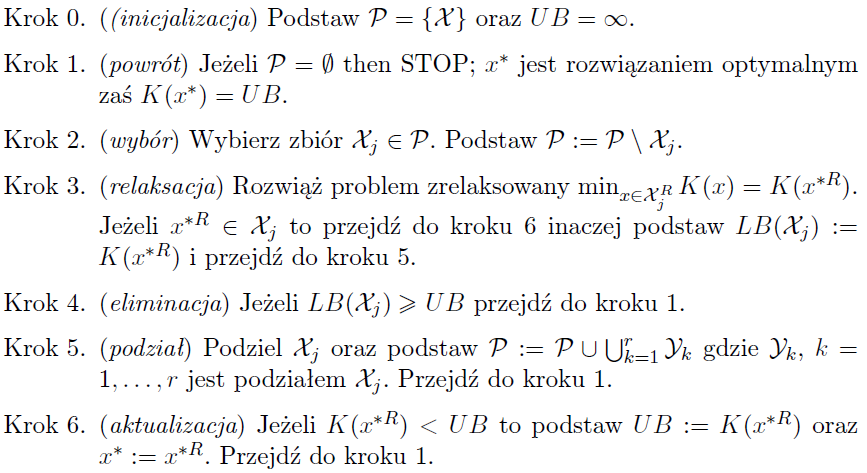
\includegraphics[width=1\textwidth]{alg.png}
	
	\subsection{Przykładowe zastosowanie}
		
		Przykładowym zastosowaniem tego schematu jest szeregowanie zadań w jedno maszynowym
		problemie z czasem dostępności, dostarczenia i możliwością przerwania zadań.
		Schemat ten implementuje algorytm Carliera, który do rozwiązywania problemów 
		zrelaksowanych wykorzystuje algorytm Schrage z podziałem.